\documentclass[10pt,conference,final,letterpaper,twoside,twocolumn,]{IEEEtran}

\usepackage{graphicx}
\usepackage{color}
\usepackage{url}
\usepackage{ifpdf}
\usepackage{hyperref}
\usepackage{xspace}

\newenvironment{shortlist}{
	\vspace*{-0.85em}
  \begin{itemize}
 \setlength{\itemsep}{-0.3em}
}{
  \end{itemize}
	\vspace*{-0.6em}
}

\usepackage{fancyhdr} \setlength{\headheight}{16.0pt}
\pagestyle{fancy} \headheight = 0pt \headsep = 25pt \fancyhf{}
\fancyhead[OC]{\bf {\it \footnotesize{Jha et al: Analysis of SAGA as
      an Access Layer for DCI}}}

\newif\ifdraft
\drafttrue
\ifdraft
 \newcommand{\amnote}[1]{  {\textcolor{magenta} {***AM: #1}}}
 \newcommand{\jhanote}[1]{ {\textcolor{red}     {***SJ: #1}}}
 \newcommand{\tmnote}[1]{  {\textcolor{blue}    {***TM: #1}}}
\else
 \newcommand{\amnote}[1]{}
 \newcommand{\jhanote}[1]{}
 \newcommand{\tmnote}[1]{}
\fi

\newcommand{\dn}{\vspace*{0.33em}}
\newcommand{\dnn}{\vspace*{0.66em}}
\newcommand{\dnnn}{\vspace*{1em}}
\newcommand{\uppp}{\vspace*{-1em}}
\newcommand{\upp}{\vspace*{-0.66em}}
\newcommand{\up}{\vspace*{-0.33em}}
\newcommand{\shift}{\hspace*{1.00em}}

\newcommand{\T}[1]{\texttt{#1}}
\newcommand{\I}[1]{\textit{#1}}
\newcommand{\B}[1]{\textbf{#1}}
\newcommand{\BI}[1]{\B{\I{#1}}}
\newcommand{\F}[1]{\B{[FIXME: #1]}}
\newcommand{\TODO}[1]{\textcolor{red}{\B{TODO: #1}}}

\begin{document}

\title{Towards Standards-Based Interoperabilty: Analysing SAGA as the
  Access Layer for OCCI backed Cloud Infrastructures}

\author{Andre Merzky$^{1}$, Thijs Metsch$^{3}$, Shantenu Jha$^{*1,2}$\\
  \small{\emph{$^{1}$Center for Computation \& Technology, Louisiana State University, USA}}\\
  \small{\emph{$^{2}$Rutgers University, USA}}\\
  \small{\emph{$^{3}$Platform Computing, Germany}}\\
  \small{\emph{$^{*}$Contact Author \texttt{sjha@cct.lsu.edu}}} }

\maketitle

\section*{Abstract} {\it Distributed infrastructures have been used by
  many applications to advance understanding in their disciplines.
  Grids are an established DCI infrastructure for distributed
  applications; clouds are an important emerging infrastructure. It is
  imperative that the lessons from the Grid experience be transferred
  as infrastructure evolve and extend to incorporate the Cloud
  paradigm.  One such lesson from the Grid experience is that,
  standards have played an important and leading role, by ensuring
  application and system level interoperability~\cite{saga_gin}, so
  that the required usage modes are (a) supported by the range of
  production grids available, and (b) that distributed application are
  able to scale beyond the boundaries of any single production
  grid. %~\cite{grid_scale_out}.
  This working/white paper motivates the need for application-level
  Cloud-Cloud and Cloud-Grid interoperability, provides a model for
  standards-based approach to such interoperability and analyses the
  advantages of an application-level interoperability to two important
  application classes: next-generation sequencing data (analysis) and
  ensemble-based simulations.}

% such interoperability, and discusses one (of many) possible
% approaches, with the significant distinction of focusing on standards.


%  Clouds are increasingly used to complement and expand the set of
%  infrastructures for distributed applications.  In parallel, efforts
%  to expand application and system level interoperability from grids
%  towards clouds are emerging.  


\section{Introduction}


\label{sec:intro}
 

 % Outline:
 % 
 % - Why Interoperability? [Cloud-Grid, Cloud-Cloud] discuss using
 %   Application exemplars
 %
 % - How? discuss ALI vs SLI, fast-track vs deep-track
 %
 % - What? We propose - using SAGA on OCCI -- which is ALI using SLI
 %   (protocols)
 %
 % - This document discusses how we will implement and architect our
 %   approach, the advantages inherent in our approach from an
 %   applicaiton point-of-view


 Distributed infrastructures have been used by many applications to
 advance understanding in their disciplines.  The requirements and
 characteristics of applications that motivate the usage of
 distributed infrastructures are very broad, and most often differ
 from regular, HPC and HTC type applications in several fundamental
 ways.  Distributed applications often need to be designed for more
 than simple peak-utilization, e.g., the number of coupled tasks that
 need to be completed within a time window.  Equally important,
 distributed applications have a much broader range of usage
 modes~\cite{dpa-paper}.

 In particular for grids as one possible DCI infrastructure for
 distributed applications, standards have played an important, and in
 fact a leading, role by ensuring application and system level
 interoperability~\cite{gin,saga-gin}, so that the required usage
 modes are (a) supported by the range of production grids available,
 and (b) that distributed application are able to scale beyond the
 boundaries of any single production grid~\cite{grid_scale_out}.

 Clouds are increasingly used to complement and expand the set of
 infrastructures for distributed applications.  In parallel, efforts
 to expand application and system level interoperability from grids
 towards clouds are emerging.  This paper motivates the need for such
 interoperability, and discusses one (of many) possible approaches,
 with the significant distinction of focusing on standards.

 The remainder of the paper is structured as follows: the next section
 (\ref{sec:interop}) discusses different forms of interoperability,
 and two exemplary application use cases which can benefit from
 grid-cloud interoperability.  We then shortly introduce SAGA
 (section~\ref{sec:saga}) and OCCI (section~\ref{sec:occi}).  Central
 to this paper, we discuss different ways toward standards based
 grid-cloud interoperability in section~\ref{sec:interop}, and map
 those to our example use cases.  We conclude the paper in
 section~\ref{sec:conc} with a short discussion about alternative and
 complementary efforts.

\section{Interoperability}
\label{sec:interop}

\subsection*{Why Interoperability?}

 \jhanote{Amongst other things, (i) support collaborative science,
   (ii) interoperable-hybrid infrastructure helps exploit
   advantages of both}
   

 \subsection*{Multiple Approaches to Interoperability}
 
 There are two major approaches to allow applications, such as those
 described above, to interoperably use DCIs: system level
 interoperability (SLI) and application level interoperability (ALI).
 SLI is the (often standards based) approach to federate multiple DCIs
 on middleware and operational level, and to allow applications to use
 the combined set of resources as if it were a single DCI.  That
 implies the exchange of accounting, authorization, authentication,
 logging, brokering and resource management information, and others,
 on system level.  Very often, SLI is implemented as delegation from
 on DCI to the other.

 ALI on the other hand does not require any activity on infrastructure
 level at all, but instead relies on the ability of the application to
 utlilize multiple independent DCIs at the same time.  While ALI is
 usually easier to achieve, it typical increases the burden on the
 application layer with the task to abstract the differences between
 DCIs.  Further, ALI based systems are inherently less sophisticated
 and less complete than SLI based systems -- for example, data
 transfer across DCI boundaries will need to be routed via the
 application layer, accounting can't be managed on application layer
 at all, etc. In addition to two application examples discussed
 earlier, there exist many other applications that can benefit from
 ALI~\cite{fgcs-interop}.
 
 \subsection*{Grid Interoperability and Standardization}

 The very idea of grid computing has been founded on the idea of
 interoperability -- otherwise the original grid vision of pervasive
 compute power from a wall plug would be impossible from the
 beginning~\cite{blueprint}.  We have all been learning the hard way
 though that 'the grid', as a *single* pervasive entity, does not
 exist, and likely is not achievable, nor desirable -- too different
 are the application requirements to computing (and data management,
 and communication) so that an all-sufficient grid infrastructure
 would be too complex to design, implement, and
 operate~\cite{ogsa-use-cases}.  Instead, a wide variety of grid
 middleware systems and grid infrastructure deployments emerged, more
 or less specifically taylored to the needs of certain application and
 user requirements.  However, at least in academia, standards have
 always been playing an important role for grid computing, as it was
 soon understood that interoperability between different grids was
 difficult to achieve without standardization, if at all~\cite{...}.

 There are however more boundary conditions to interoperable grid
 infrastructures than standardized interface definitions and
 protocols: operational concerns, and in particular security and
 accounting issues, have shown to be a major impediment to really
 usable grid SLI~\cite{gin-usecases}.  The efforts of OGF groups like
 HPC-BP, GIN and PGI are, to a large extent, revolving around those
 issues, trying to separate interoperability from
 interoperation~\cite{gin-papers, ogf-www}.

 While not being able to solve any system level interoperational
 issues, ALI approaches have shown to provide similar levels of rid
 interoperability with significantly less effort, and improved end
 user experience.  We have been showing that SAGA based ALI is one
 possible incarnation of application level grid interoperability, with
 the additional benefit of being standards based~\cite{saga-gin,
 mandelbrot-www}.

\subsection*{Cloud Interoperability and Standardization}

 The need for cloud standards and interoperabilty can be appreciated
 from a technology as well as an application perspective. One example
 of a technology pull for standardization is provided by need for
 interoperability across {\it Specialized Clouds}, i.e., emerging
 customized clouds that support specific capabilities or services,
 analagous to HPC grids (TeraGrid) versus HTC grid (Open Science Grid)
 or Data Grids (EGEE).  The application push can be understood by the
 imperative to operate on massive amounts of data {\it in situ}, which
 in turn involves computation across heterogeneous distributed
 platforms as part of the same application.  For example, the Earth
 System Grid involves peta to exa-bytes of data, and one cannot move
 all data (given current transfer capabilities), nor compute at a
 centralized location.  In addition, there exist a wide range of
 applications that have decomposable but heterogeneous computational
 tasks.  Some of these tasks are better suited for traditional grids,
 or on a specific cloud over another, e.g., applications in the LEAD
 project, some workloads are better placed on a data cloud whilst some
 should optimally be located on regular clouds or even grids, due to
 different data-compute affinity requirements amongst the tasks. 

 It is worth mentioning that most \I{existing} efforts at cloud
 interoperability are at the service managment, cloud network or
 federation level, and thus SLI.  Only few standard based efforts
 exist on that level.  Notably, OCCI aims to provide remote management
 protocol and API specification for IaaS clouds.  It complements
 related standards of SNIA and DMTF, while competing with more
 proprietary approaches such as those from VMware or Amazon.  Even
 fewer efforts target grid-cloud interoperability on system level: the
 inherent technology devide is considered a significant impediment for
 grid-cloud SLI.  A notable exception is the DCIFed working group at
 OGF~\cite{dcifed-www}.
 
 % Even fewer interoperability efforts exist on cloud-ALI, and are based
 % on non-standardized APIs (such as Amazon's EC2-API).  We aim to
 % provide the first such application-level interoperability built on
 % the back on existing community standards and efforts.  

 OCCI has been able to gather significant community and industry
 support and uptake, e.g., early uptake in community driven cloud
 stacks (OpenNebula, OpenStack, Eucalyptus etc).  OCCI is however, a
 REST-ful protocal with limited API capabilities rather than a full
 blown interface definition, and will thus, at least initially,
 experience different, likely non-interoperable implementations. OCCI
 will thus make cloud interoperability easier, but not simple {\it for
   the application developer or user}.  But by integrating SAGA with
 OCCI we can provide broad coverage for applications, i.e., SAGA as
 the application/client API to OCCI should be able to shield an
 application from the specific OCCI implementations as well as provide
 grid-cloud interoperability.


 \subsection*{Applications Requiring Grid-Cloud Interoperabilty}

 To motivate the further discussion in this paper, we shortly describe
 two real-world use cases which have been driving grid and cloud
 interoperability efforts in the recent past.  One is a data-intensive
 application -- a genome analysis tool BFAST; the other is more
 compute intensive -- ensemble based MD simulations.
 
 \BI{BFAST}: Next-Generation gene Sequencing (NGS) machines produce
 significantly larger amounts of data compared to early sequencers.
 In addition to the challenge of data-management that arise from
 unprecedented volumes of data, there exist the important requirement
 of effectively analyzing the data.  In this paper, we use
 BFAST~\cite{bfast2009,bfast2009b} -- genome-wide mapping application,
 as a representative example of the typical analysis that is required
 on data from NGS machines.  BFAST is representative of a diverse set
 of applications aimed at genome-wide analysis.
 
 Its features include i) a requirement of input files containing
 sequence information of a reference genome or short reads from NGS
 platforms, ii) a production of output files that is generally written
 with a format that is successively injected to another tool as input.
 These aspects, along with a huge variation in the data volume in
 input, output, or temporary files, often require that the execution
 environment should scale-up (range of parallel, multi-threading
 executions on a single resource), as well as scale-out (range of
 distinct resources and distribution).
 
 BFAST initially requires a reference genome sequence and NGS
 generated short reads, and prepares input files with pre-defined
 formats.  Then, the program indexes of the reference genome, searches
 for Candidate Alignment Locations (CALs) and local alignment of CALs,
 and post-processes these alignment results, which at the end produces
 the mapping of the billions of short reads onto the target reference
 genome.  Among these steps, the indexing, matching, and local
 alignment steps are the most computationally demanding -- compute
 requirements generally scale with the size of the reference genome as
 well as the number of short reads.

 \BI{Ensemble-based MD simulations} are commonly used bio-molecular
 simulation approaches, used to enhance the sampling and convergence
 for biomolecular simulations.  Ensemble based approaches represent an
 important and promising attempt to overcome the general limitations
 of insufficient time-scales, as well as specific limitations of
 inadequate conformational sampling arising from kinetic trappings.
 The fact that one single long-running simulation can be substituted
 for an ensemble of simulations, makes them ideal candidates for
 distributed environments.  This thus provides an important general
 motivation for researching ways to support scale-out and thus enhance
 sampling and to thereby increase the ''effective'' time-scales
 studied. 
 
 In Ref.~\cite{ccgrid10, cloudcom10}, we implemented the compute
 and coordination pattern represented by \I{replica-exchange} on
 different Clouds -- IaaS (Eucalyptus and Nimbus-based) and PaaS
 (Azure), by extending the SAGA-based Pilot-Job (BigJob) framework to
 utilize the native abstractions provided by these Clouds, e.g., such
 as worker roles on Azure and affinity groups (at the data-center
 level).

\subsubsection*{Understanding the Execution Patterns of the
   Applications}

 The ensemble-based simulations have two primary modes of execution.
 In the zero-coupled ensemble N ensemble run independent of each
 other; they run to completion which is typically a fixed number of
 steps. Although the runs are independent, the analysis is not always
 independent. In the loosely-coupled ensemble mode, the individual
 replicas run for a fixed number of steps, before exchanging state
 information; the exact length of execution is also not well defined
 as often the exchange step is a stochastic variable.  There are
 multiple variants of the exchange algorithm, and depending upon which
 version is employed, the pairing between replicas might be
 time-dependent (dynamic determined) or independent (static).

 The BFAST application in contrast is a data-intensive application; it
 can be used to employ different levels of parallelism -- either fine
 grained parallelism (at the thread level) or multiple concurrent
 tasks.  There are two important data-sets that BFAST operates on: the
 reference genome and input sequence data (from experiments). The
 reference genome is processed to yield {\it index files} set-up in a
 certain format, so as to exploit certain types of parallelism. The
 input sequence data is in many millions of small (read) files.
 Typically BFAST runs on a single processor, multiple-threads; however
 due to IO sub-systems constraints, utilizing distributed resources is
 can bring about performance improvements; additionally using
 distributed resources is often be often beneficial from a
 data-transfer and management issue.

 There are multiple reasons why BFAST may use Cloud resources; it
 requires a reference geneome which are often community resources.
 

\section{SAGA: the Simple API for Grid Applications}
\label{sec:saga}

 SAGA has been presented and discussed in detail
 elsewhere~\cite{sagapub...}, and has been used for application level
 interoperability before~\cite{sagainterop...}.  This section shortly
 summarizes the relevant findings.

 SAGA is an acronym for "Simple API for Grid Applications". As the
 name suggests, a simple API which facilitates the development and
 execution of distributed applications on most types of distributed
 infrastructure.  Modern distributed computing environments are very
 complex infrastructures, and allowing applications to make use of
 these complex systems is not trivial.  By defining a simple API, one
 requires those complexities to be dealt with at levels other than
 application code and development.  Simplicity of the interface is the
 primary design principle and objective of SAGA.  The fact that SAGA
 is a (set of) OGF standard(s)~\cite{sagaspecs...} ensures the
 community-wide adoption and stability of the API.  Functional goals
 of SAGA are:

 \begin{enumerate}

  \item Provide a stable programming interface to distributed
  application programmers and tool developers
 
  \item Shield developer from heterogeneous and evolving
  infrastructures and middlewares

  \item By providing the building blocks to distributed and remote
  operations enable the expression of high-level abstractions and
  support of distributed application requirements

 \end{enumerate}

 The SAGA standardization effort is closely syncronized with other
 specification and community efforts, within and outside of OGF.  In
 particular, OGF groups ensure that SAGA semantics map well to lover
 level specifications, such as JSDL, BES, GridFTP, etc.   But also,
 and possibly more importantly, it is now widely and independenly
 acknowledged~\cite{XD,EGI,UMD,Naregi} that a uniform, simple and
 stable access layer is neccessary (but not sufficient) to improve end
 user experience on distributed computing infrastructures, and that
 SAGA can indeed play that role for a specific set of use cases.  As
 such, SAGA is now integral part of the GIN (Grid Interoperation Now)
 community effort, and also plays an active role in current efforts
 like OGF's PGI group. % and US's XD proposals.
  
 Although SAGA is foremost an API, the SAGA distributions support end
 users in a variety of ways.  In particular, the SAGA distributions
 also include command line tools implemented via the SAGA API, and
 higher level libraries for common distributed programming patterns,
 also basing on the SAGA API.


 \subsubsection*{The Price of Simplicty\cite{sagaprice}}

  There are three main costs associated with an ALI approach like
  SAGA, which tries to provide a simple, stable, concise and
  consistent layer on top of a very dynamic and exceedingly complex
  set of infrastructures.  First, there are performance penalties.  We
  show in~\cite{sagaperf} that those are, for almost all of our target
  use cases, acceptable, or at least manageable.  Second, almost all
  abstractions in IT are leaking once the underlying systems become
  too complex~\cite{leaky_abstractions}.  Despite trying very hard to
  pinpoint the SAGA API semantics, and to avoid abstraction leakage,
  we have to face this uphill battle.  Third, and even more
  importantly, there remains the fact that the SAGA layer itself, i.e.
  the SAGA implementation, is an very complex component.  Although
  that fact is well understood, and an intentional design artefact, it
  needs dealing with on several levels.  Amongst others, it is
  becoming increasingly clear that SAGA deployment needs to be dealt
  with at levels distinct from the SAGA end user, namely at the DCI
  provider level~\cite{UMD,XD,TG}.


 \subsubsection*{SAGA in the Clouds}

  Although the SAGA acronym contains the G-word, it is, first of all,
  an API for programming distributed applications.  As such, it is
  suitable for classical grid and non-grid DCIs, but just as well
  usable for cloud infrastructures~\cite{sagacloud...}.  In particular
  in respect to the 'leaky abstractions' mentioned above, one has to
  acknowledge that the dynamic resource provisioning aspects of clouds
  have certain implications for the semantic interpretation of the
  higher level SAGA API.  For example, resource life time assumptions
  which are valid on Grids have a very different meaning in clouds.
  While we have shown~\cite{sagacloud...} that SAGA can handle fairly
  simple scale-out scenarios onto clouds rather well, it will require
  some additional API semantics to more efficiently, and
  transparently, use cloud resources.  Interestingly, those cloud
  requirements are \I{very} similar to requirements SAGA has recently
  received from the grid application community.  For example, the SAGA
  based pilot-job implementation 'BigJob'~\cite{bigjob} is, at the
  moment, one of the dominant usage modes for TeraGrid and DEISA
  resources, for the SAGA community.  Application level resource
  allocation and reservation paradigms like pilot job and the cloud's
  dynamic resource provisioning paradigms have, on API level, many
  things in common, so that it seems sensible to expand
  SAGA\footnote{The SAGA API is, by design, extensible.  In fact,
  multiple SAGA extensions have already been defined, and are
  undergoing the same standardization process as SAGA itself.} by a
  relatively generic resource management API.  It must be noted that
  SAGA's notion of resource management has \I{almost nothing} to do
  with resource management on infrastructure level, but rather is an
  expression on how an application is discovering and allocating
  required resources.
  

\section{OCCI: the Open Cloud Computing Interface}
\label{sec:occi}

 The Open Cloud Computing Interface consist of a set of open
 community-driven specifications, provided under the umbrella of the
 Open Grid Forum and consists of a RESTful \cite{REST_Fielding}
 protocol and accompanying service interface definitions.  It targets
 all kinds of management tasks based on a Resource Orientated
 Architecture (ROA) \cite{RR2007}.  OCCI was originally initiated to
 create a remote management API for IaaS model based Services,
 allowing for the development of interoperable tools for common tasks
 including deployment, autonomic scaling and monitoring of virtual
 machines (IaaS).  It has since evolved into a very flexible protocol,
 with a strong focus on integration, portability, interoperability and
 innovation, while still offering a high degree of extensibility.  The
 current release of the Open Cloud Computing Interface is intented to
 also cater to many other models in addition to IaaS, including PaaS
 and SaaS\footnote{\url{http://www.occi-wg.org/}}.

 The OCCI specifications fall into three categories: the OCCI Core,
 OCCI Renderings and OCCI Extensions.  Three OCCI documents exist and
 are being implemented by various implementations:
 
 \begin{itemize}
 
  \item The \B{OCCI Core} specification consists of a single document
  defining the OCCI Core Model. That model can be expanded via
  \I{extensions}, and can be interacted with via \I{renderings}.

  \item The \B{OCCI HTTP Restful Rendering} specification describes
  one particular rendering of the OCCI Core Model.  The HTTP Restful
  Rendering describes an HTTP based RESTful API to interface with
  services which implement the OCCI Core Model.  Other renderings are
  feasable and could interact with the same instance of the OCCI Core
  Model.  
 
  \item The \B{OCCI Infrastructure} specification is an extension of
  the OCCI Core Model which allows to apply the OCCI model to the IaaS
  domain. Other documents could describe other ways and means of
  extending the Core Model, for other elements of the IaaS domain, or
  for the PaaS and SaaS domains.  
  
 \end{itemize}

 Future releases of OCCI may include additional renderings like JSON,
 or additionale extensions, e.g. basing on OVF.

 \subsubsection{OCCI in Relation to Other Cloud Standards}

 Since OCCI is an RESTful protocol and service interface, it can build
 upon all the features defined by HTTP. This includes mechanisms for
 authentication and authorization, cache-mechanisms, content-type
 definitions and discovery capabilities.
 
 Another guiding principle for OCCI is to make use of existing
 standards and specifications where appropriate.  For example, OGF's
 OCCI working group and the Storage Networking Industry Association's
 (SNIA)\footnote{\url{http://www.snia.org/}} Cloud Data Management
 Interface (CDMI) working groups have collaboratively ensured that
 both specifications are interoperable with each other.  CMDI can be
 used to create, retrieve, update and delete data elements in a Cloud
 offering. References to data elements, which result from CDMI service
 interactions, can directly be used when interacting with an OCCI
 compatible service.
 
 Similarly, OGF's OCCI working group and the Distributed Management
 Task Force's (DMTF)\footnote{\url{http://www.dmtf.org/}} Open
 Virtualization Format (OVF), see \cite{CDG+2009}, can be easily
 integrated through the use of the OCCI resource type 'Link'.  Where a
 provider wishes to supply an OVF representation of a client's
 resource instance(s), they can do so by associating the instance(s)
 with a mirror representation, with the serialisation/rendering format
 being OVF.
 
 The OCCI working group is also closely working together with other
 groups inside the Open Grid Forum. The Distributed Computing
 Infrastucture Federation (DCI-fed) working group focuses on the
 creation of models and APIs for setting up distributed federated
 computing environments. The OCCI working group further plans to use
 Standards like the Distributed Resource Management Application API
 (DRMAA) for common Job operations on clusters, via the OCCI protocol.
 
 All those efforts will, upon adoption, simplify service-level cloud
 interoperability efforts.  The landscape of cloud based DCIs is,
 however, evolving very fast and dynamically, and it remains to be
 seen what OCCI extensiont will be required to cater to emerging
 federation use cases.
 
 
\section{Grid-Cloud interoperatbilty}
\label{sec:gcinterop}
 
 The next paragraphs describe our proposed approach on Cloud-Grid
 interoperability. We propose elements of a standards based
 architecture which provides SLI where appropriate, and ALI where
 needed, to allow to interoperably span grid and cloud based DCI's.
 We then demonstate the usability of that architecture by applying it
 to the previously described use cases.
 
 \subsection{(A) SLI/OCCI for job submission endpoints, SAGA as client}
 
 On the simplest level, OCCI could be used in its reduced capability
 as job submission protocol (see fig~\ref{fig:arch1}): it would be
 relatively straight forward to, for example, provide a cluster job
 submission service based on the OCCI protocol. Such an approach would
 allow applications and tools to uniformly submit jobs to cluster and
 cloud resources. For example the DRMAA specification as previously
 mentioned could be used to model the extensions needed for OCCI.
 
 Along those lines, a SAGA-OCCI adapter could implement job submission
 to OCCI endpoints, while making extensive usage of OCCI's automatic
 discovery and billing mechanisms. To ensure interoperability the
 capabilities of the job submission interface in OCCI would require
 that an extension be added to the OCCI specification.
 
 \begin{figure}[h!]
  \center{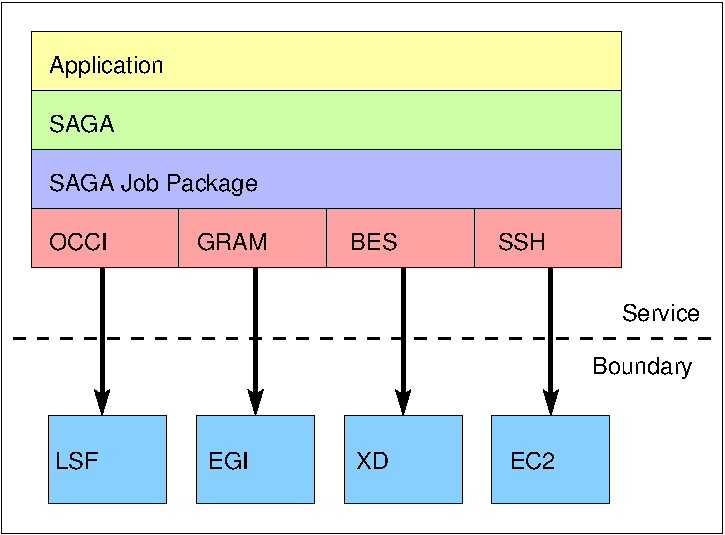
\includegraphics[width=0.35\textwidth]
  {figures/arch_1.pdf}}
  \caption{\footnotesize\label{fig:arch1} \B{Using OCCI for job 
     submission} allows for ALI with traditional grid infrastructures.  
     While this scenario focuses on job submission, the discussion 
     applies just as well to scenarios focusing on data access or 
     communication.}
 \end{figure}
 
 Although, the scenario is technically straight forward, and can very
 well co-exist with existing standards based job submission
 approaches, it would at some level have to compete with other, well
 established job submission mechanisms. However, a major advantage of
 using OCCI over standards like OGSA-BES or similar would be the usage
 of RESTful interfaces over SOAP based protocols. Additionally, the
 idea of having one protocol (syntax and a way of expressing the
 semenatics) to talk to more then one service is an attractive
 one. OCCI will not only be used for the Job submission but also for
 accesing Data (like NoSQL Databases and MapReduce File Systems),
 Authentication (using the HTTP features) and Integration (bonding
 different Interfaces together using one Procotol).

 \subsection{(B) SLI/OCCI for IaaS resource provisioning, ALI/SAGA 
 for resource access}

 IaaS based clouds allow to create virtual machine instances on
 demand, and thus allow to provision resources for applications on the
 fly.  Pure VM instances are, however, not sufficient to run
 applications: the application processes need to be started on these resources,
 and need to be able to interact with other application components on
 other resources (data transfer, coordination, etc).  A common way to
 achieve this is to bootstrap the VM instances in such a way that some
 kind of midleware is provided on these resources, which can then be
 used by the application to get enroled as described.  The default on
 many IaaS coulds is to enable ssh access for VM instances, but other
 access mechanisms are possible and available.

 In order to get VM instances configured in such a way, one needs to
 either add an extension to OCCI which allows to describe the VM's OS
 and middleware stack in some detail; or one uses OVF inside OCCI to
 point to pre-configured VM images which are used to directly boot
 such pre-configured VM instances.  Both cases would be fully
 standards based, portable between different (OCCI compliant) cloud
 providers, and would be able to create and application environment
 which spans multiple cloud and grid DCIs transparently.
 
 Since SAGA features a rich set of adapters to talk to Grid
 Middlewares (such as DRMAA and BES adaptors), it seems perfectly
 feasable to use OCCI to instantiate resources in a cloud DCI, in such
 a way that the VM instances are configured to run one of the grid
 middlewares supported by SAGA.  In some sense, OCCI is thus used to
 instantiate a virtual grid (or components thereof) on the cloud DCI,
 on the fly.  SAGA can then be used by the application to utilize
 those resources as it usually does (on pure grid resources).  That
 scenario is shown in fig.~\ref{fig:arch2}.

 \begin{figure}[h!]
  \center{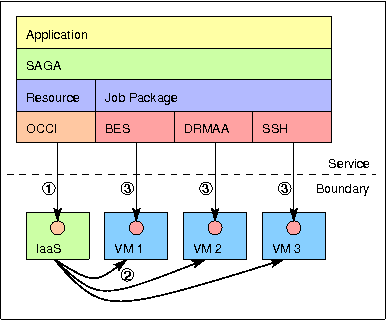
\includegraphics[scale=0.5] {figures/arch_2.png}}
  \caption{\footnotesize\label{fig:arch2} \B{Using OCCI for IaaS resource provisioning}: 
     (1) SAGA uses OCCI to request resources at an IaaS Service; 
     (2) the IaaS service uses OCCI to provision those resources 
          with a standardized job submission endpoint; then 
     (3) SAGA uses the respective job submission protocol to utilize 
     the provisioned resources.}
 \end{figure}

 SAGA is, at the moment, only offering very rudimentary means to
 specify resource lifetime requirements, and is thus inadequately
 equipped to implement the architecture shown.  The OGF SAGA working
 group is, however, working on a resource management package which
 will address exactly those issues.


 \subsection{(C) Combine SAGA and OCCI to create a PaaS Offering}

 The above architectures utilize OCCI in its current main usage mode,
 as management protocol for IaaS cloud resources.  We have seen
 in~\ref{fig:arch3} that OCCI can potentially be used to enrol
 (potentially complex) virtual infrastructures on IaaS clouds, such as
 virtual clusters, or virtual grids.  There are, however, two elements
 missing to turn those virtual infrastructures into PaaS offerings:
 first, we miss an API which would allow to code 'native' applications
 against that virtual infrastructure; secondly, OCCI is currently
 missing the ability to enrol those applications on the virtual
 infrastuctures.  Current PaaS offerings such as "Google's AppEngine"
 or Amazon's WebServices (e.g., Amazon Queuing-service), Azure, are
 prominent examples of how those capabilities could be rendered.

 \begin{figure}[htb]
  \center{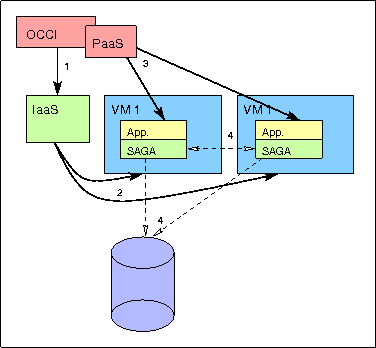
\includegraphics[scale=0.5]
  {figures/arch_3.png}}
  \caption{\footnotesize\label{fig:arch3} \B{PaaS offering using 
      OCCI and SAGA}: 
      (1) a user tool uses OCCI to register a workload 
          description and input data with an PaaS service; 
      that service 
      (2) uses OCCI to provision application data to virtual storage; 
      (3) uses OCCI to provision compute resources; and
      (4) uses OCCI to provision the application workload on these resources; 
      (5) the application workload uses SAGA to access the virtual
          infrastructure.}
 \end{figure}

 We argue that SAGA can be used to address the first concern, and that
 a SAGA based service, utilized by an OCCI extension for application
 deployment, is one way to address the second concern: SAGA
 applications (i.e. distributed application coded against the SAGA
 API) have been shown to allow to express a wide variety of
 distributed programming paradigms, and to utilize physical and
 virtual distributed infrastructures -- SAGA would thus be able to
 address the first missing element, an 'application API' for the PaaS
 infrastructure.  But also it has been shown that SAGA can be used to
 enrol applications on a wide range of infrastructures, thus a SAGA
 based application deployment service could address the second missing
 PaaS element, when enacting a respective OCCI application deployment
 extension.


 \subsection{ALI versus SLI, revisited}

 All three scenarios above allow for SAGA based applications to
 utilize virtual IaaS or PaaS infrastructures.  It would thus
 immediately allow to expand SAGA based ALI, as described in
 section~\ref{sec:interop}, towards OCCI based infrastructures.

 As the OCCI deployment of virtual resources in scenario (B) and (C)
 has additional control over the deployed middleware stack, those
 scenarios also allow for SLI scenarios: the created virtual
 infrastructure can on the fly be configured in a way that it allows
 for system level interoperation with other (virtual and physical)
 distributed infrastructures.  One could, for example, imagine the
 system level integration of remote data sources into the newly
 created virtual environments, to support data intensive applications
 on those.

 \begin{table}[thb]
  \centering
  \footnotesize
  \begin{tabular}{|p{20mm}|p{16mm}|p{16mm}|p{17mm}|}
   \hline
                          & \B{Scenario (A)}      & \B{Scenario (B)}      & \B{Scenario (C)}       \\
                          & \I{Job Subm. via \newline SAGA/OCCI} 
                                                  & \I{IaaS through\newline SAGA/OCCI} 
                                                                          & \I{PaaS via\newline
                                                                               SAGA/OCCI} \\\hline\hline
   Application API        & SAGA                  & SAGA                  & SAGA                   \\\hline
   PaaS Interface         & --                    & --                    & OCCI                   \\\hline
   IaaS Interface         & --                    & OCCI                  & OCCI                   \\\hline
   Job Submisison\newline Interface
                          & BES, DRMAA, SSH, OCCI & BES, DRMAA, SSH, OCCI & BES, DRMAA, SSH, OCCI  \\\hline
  \end{tabular}
  \caption{\label{table:standard-function}Table listing the different
  levels at which integration of OGF Standards can take place.  See
  figures~\ref{fig:arch1}-\ref{fig:arch3} for more details.}
 \end{table}

 It must be noted, however, that those scenarios are, for the time
 being, at the functional edge of OCCI's scope -- they require rather
 sophisticated means to describe the virtual infrastructure (including
 its software stack and middlware configuration) in fine detail before
 its instantiation. Since OCCI first focuses on portability and
 interoperability, the capabilities described in the specification are
 limited but enough to enable these. The extension mechanism of OCCI
 allow more detailes to be transmitted to Service Providers -- for
 example, extensions to the embedded OVF format can be used to
 describe infrastructure requirements in more detail.

 During the EU project RESERVOIR
 \footnote{\url{http:/I /www.reservoir-fp7.eu/}}, such OVF extensions
 have been defined which can be used to described such setups in
 details \cite{comsware09}.  It has been shown that it is possible to
 request more complex setups, like requesting a complete Sun Grid
 Engine \footnote{now Oracle (\url{http://www.oracle.com/}) or Univa
 Grid Engine (\url{http://www.univa.com})} cluster which then could be
 used by SAGA.


 \subsection{Mapping the use cases}

 We have outlined three different ways to allow applications to
 interoperate accoss physical and virtual (grid and cloud)
 infrastructures.  We will shortly map our two application use cases
 to these architectures, to further underpin the usability of the
 proposed architectures.  While this is \F{circumstantial?} evidence
 at best, we hope it helps to better illustrate the power and
 flexibility of the proposed standards based approach on grid-cloud
 interop.

 \subsubsection*{(A) SLI/OCCI for job submission endpoints, SAGA as client}

 The first use case is conceptually very simple: integrating OCCI as
 an standardized job submission mechanism to (already provisioned)
 IaaS resources allows our applications to transparently scale-out to
 cloud resources.  The Ensemble Simulation use case would additionally
 require some means of data exchange between the distributed
 application components -- that is relatively easy to solve on
 application level.  The BFAST application use case would need to make
 use of similarly standardized data access mechanisms to be able to
 make use of those resources.  In particular the need for data/compute
 co-location may pose a significant barrier in this case, as that
 usually cannot be efficiently provided without system level support.
  

 \subsubsection*{(B) SLI/OCCI for IaaS resource provisioning, ALI/SAGA for
 resource access} 

 For the application use cases, our scenario (B) is very similar to
 the previous one (A) -- the main difference is that the IaaS
 resources are now dynamically provided, which allows the applications
 to \I{dynamically} scale-up and scale-out.  While BFAST's execution
 pattern is rather static, the Ensemble Simulations can certainly make
 use of that feature at runtime~\ref{re-paper}.  Both applications
 can, however, benefit from the dynamic provisioning for overall
 runtime optimization, e.g. to meet completion deadline constraints or
 to optimize total time-to-solution.


 \subsubsection*{(C) Combine SAGA and OCCI to create a PaaS Offering}

 The PaaS scenario is the one which differs most from the default
 modus operandi of our example applications, and is thus the most
 interesting to discuss.  On the surface, there is not much change
 compared to scenario (B), only that provisioning decisions and
 actions are done by the PaaS service.  Particularly the BFAST
 application will be able, however, to benefit from the data
 provisioning step (2) shown in fig.~\ref{fig:arch3}, as that will,
 together with the on-demand infrastructure provisioning, allow for
 data-compute co-location, which enables more efficiant instatiations
 of the BFAST execution pipeline.


\section{Conclusions}

%  Although we have mapped three possible scenarios of integrating SAGA
%  and OCCI, we anticipate that the most commonly used scenario will be
%  Mode XXX, because...

%  \label{sec:conc}

% % \F{hurra hurra hurrra!}


\bibliographystyle{plain}
\bibliography{inter-cloud-grid-2011,ecmls11}

\end{document}

